% Intended LaTeX compiler: pdflatex
\documentclass[25pt, a0paper, portrait, blockverticalspace=7mm]{tikzposter}
\RequirePackage{fix-cm}
\usepackage[scaled]{helvet}\renewcommand{\familydefault}{\sfdefault}
\usepackage[T1]{fontenc}\usepackage{graphicx}\usepackage{amssymb}\usepackage{environ}\usepackage{enumitem}
\usetikzlibrary{positioning, arrows.meta, fit, calc, backgrounds}
\pdftrailerid{}\hyphenpenalty=10000\exhyphenpenalty=10000
\newcommand{\bodyfont}{\fontsize{30}{38}\selectfont\raggedright}
\newcommand{\secfont}{\fontsize{26}{32}\selectfont\raggedright}
\newcommand{\diagfont}{\fontsize{26}{31}\selectfont}
\newcommand{\diagsub}{\fontsize{22}{27}\selectfont}
\newcommand{\bignum}[1]{{\fontsize{120}{120}\selectfont\bfseries #1}}
\newcommand{\bt}[1]{{\fontsize{40}{48}\selectfont #1}}
\newcommand{\chip}[2]{{\fontsize{26}{30}\selectfont\color{#1}\,[#2]}}
\definecolor{ink}{HTML}{0B0B0B}\definecolor{ink2}{HTML}{52514E}\definecolor{accent}{HTML}{2A78D6}
\definecolor{warm}{HTML}{EB6834}\definecolor{good}{HTML}{0CA30C}\definecolor{neutral}{HTML}{F0EFEC}
\definecolor{critical}{HTML}{D03B3B}\definecolor{paper}{HTML}{FCFCFB}\definecolor{arcblue}{HTML}{0074D9}
\definecolor{arcred}{HTML}{FF4136}
\definecolor{band1}{HTML}{FDEBD3}\definecolor{band2}{HTML}{FADBD8}
\usetheme{Simple}\tikzposterlatexaffectionproofoff
\colorlet{backgroundcolor}{paper}\colorlet{framecolor}{paper}\colorlet{titlefgcolor}{ink}
\colorlet{titlebgcolor}{paper}\colorlet{blocktitlebgcolor}{paper}\colorlet{blocktitlefgcolor}{accent}
\colorlet{blockbodybgcolor}{paper}\colorlet{blockbodyfgcolor}{ink}
\newcommand{\postersubtitle}{Learning from Failure: Executable Reasoning and Hypothesis Revision}
\newcommand{\posteraffil}{University of Missouri}
\newcommand{\posterstatus}{REVIEW DRAFT V2, 19 October: for collaborator review, not for print}
\makeatletter\settitle{\centering\vbox{\color{titlefgcolor}{\bfseries\fontsize{100}{112}\selectfont \@title\par}\vspace*{0.2em}{\fontsize{50}{60}\selectfont \postersubtitle\par}\vspace*{0.25em}{\fontsize{36}{44}\selectfont\color{ink2} \@author\ \,$\cdot$\, \posteraffil \quad {\color{critical}\posterstatus}}}}\makeatother
\tikzset{stage/.style={rounded corners=8pt, draw=accent, line width=2.6pt, fill=white, align=center, font=\diagfont, inner sep=9pt},
pstage/.style={stage, dashed, draw=ink2, dash pattern=on 12pt off 7pt},
ctx/.style={rounded corners=8pt, draw=none, fill=neutral, align=center, font=\diagfont, inner sep=9pt},
flow/.style={-{Latex[length=8mm,width=6mm]}, line width=2.8pt, draw=ink2},
dflow/.style={flow, dashed, dash pattern=on 12pt off 7pt},
lab/.style={font=\diagsub, text=ink2, align=center}}
\NewEnviron{posterblock}[1]{\block{#1}{\BODY}}
\author{Chimdi Walter Ndubuisi}
\date{}
\title{LEARNING WHAT TO CHANGE}
\begin{document}

\maketitle[width=0.97\linewidth, titletotopverticalspace=10mm, titletoblockverticalspace=6mm]

\begin{posterblock}{}
{\centering\fontsize{56}{66}\selectfont\bfseries
How can a machine learn the representation and rules of new data, learn from failure, and know what to reconsider
when its explanation is not enough?
\par}\vspace{0.15em}{\centering\fontsize{28}{34}\selectfont\color{ink2}
\textbf{Representation:} what counts as an object, and which relations matter. \textbf{Rules:} what the objects do. \textbf{New data:}
neither is given in advance.
\par}\vspace{0.5em}\begin{minipage}[c]{16.8cm}
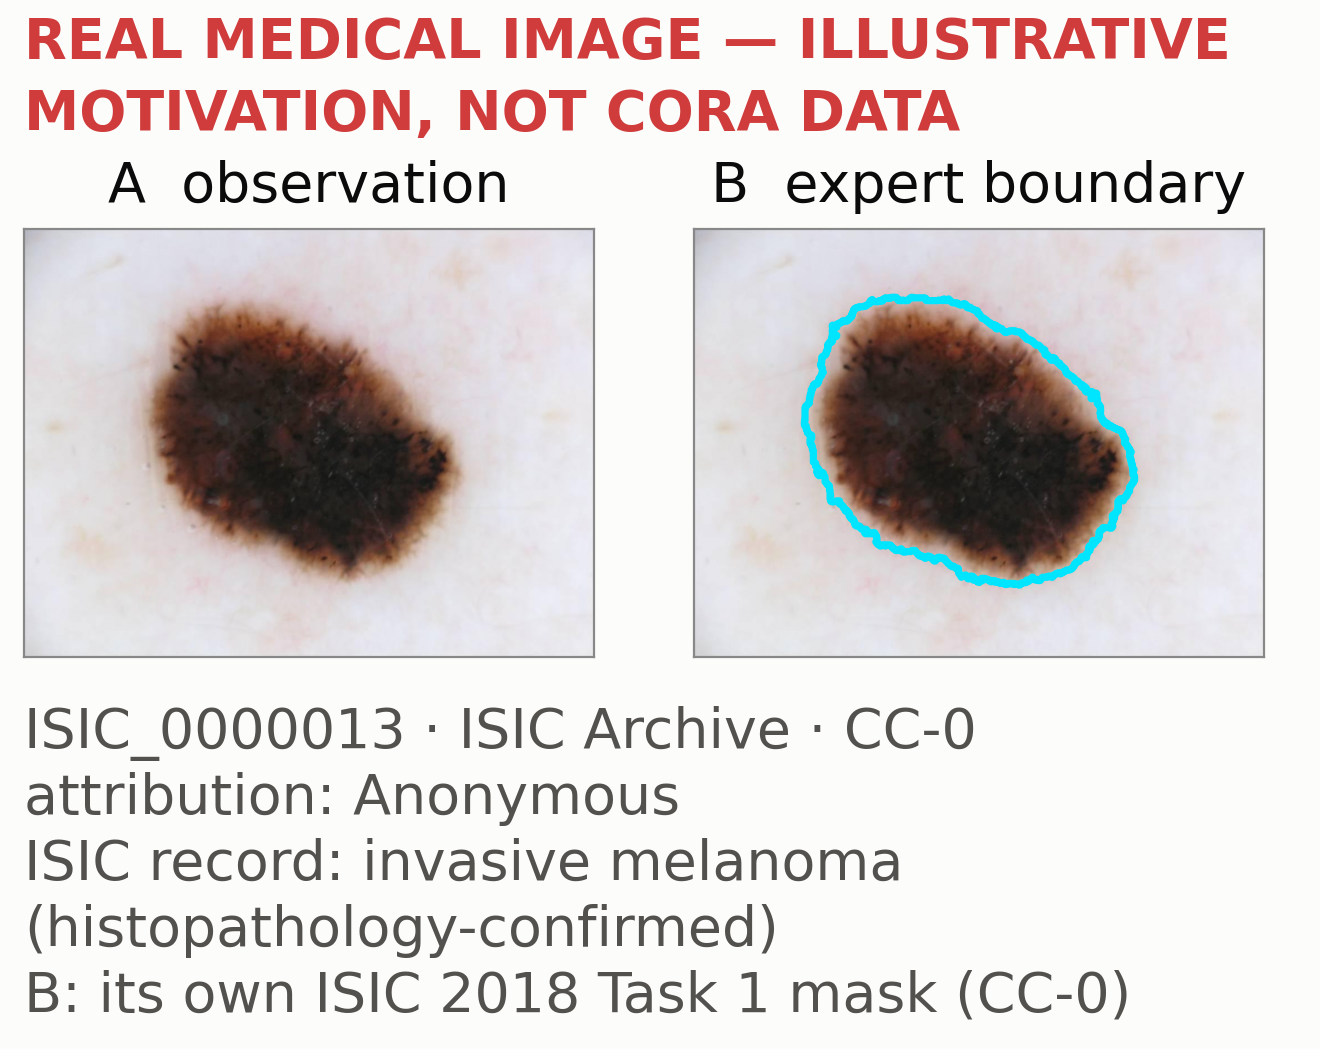
\includegraphics[width=16.8cm]{figures/fig_skin_lesion_ISIC_0000013_with_boundary.png}
\end{minipage}\hspace{0.4cm}\begin{minipage}[c]{9.9cm}
\includegraphics[width=9.893cm]{figures/fig_maize_annotated_DSC_0042_crop_x2.png}
\end{minipage}\hspace{0.9cm}\begin{minipage}[c]{10.6cm}
\centering
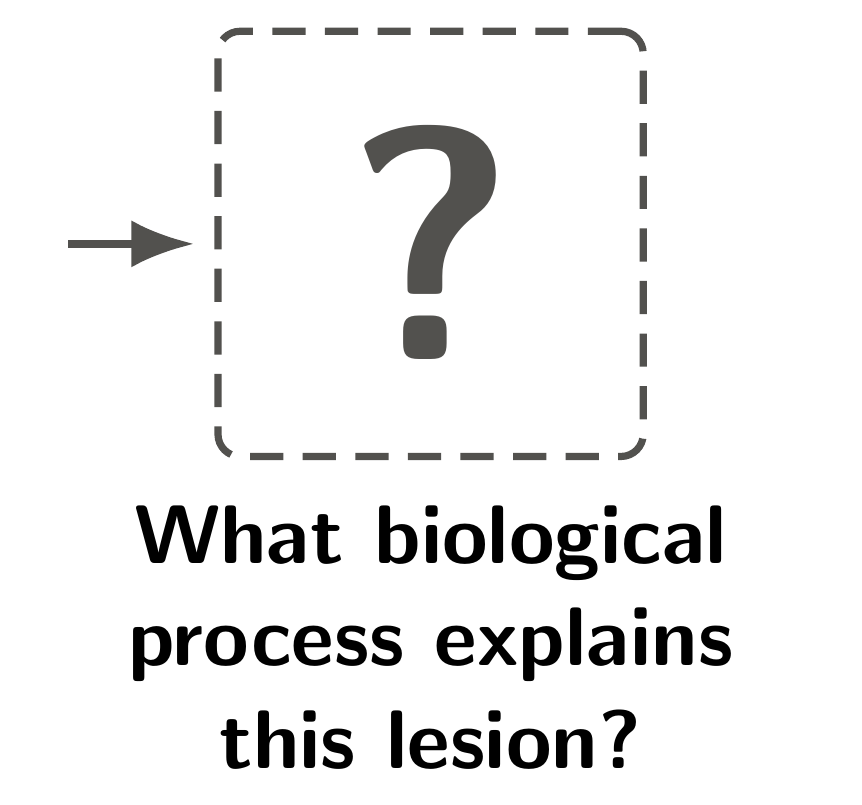
\begin{tikzpicture}
  \draw[flow] (-4.6,2.6) -- (-3.0,2.6);
  \node[pstage, minimum width=5.4cm, minimum height=5.4cm, font=\fontsize{120}{120}\selectfont\bfseries, text=ink2] (h) at (0,2.6) {?};
  \node[anchor=north, text width=10.0cm, align=center, font=\fontsize{30}{37}\selectfont\bfseries] at (0,-0.6)
    {What biological process explains this lesion?};
\end{tikzpicture}
\end{minipage}\hspace{0.9cm}\begin{minipage}[c]{35.4cm}\raggedright{\fontsize{30}{39}\selectfont
\textbf{Observe:} what is in the image?\\[0pt]
\textbf{Represent:} where is the lesion, and what are its relevant features?\\[0pt]
\textbf{Explain and test:} what biological explanation fits independent clinical, histological or molecular evidence?
\par}\vspace{0.5em}{\fontsize{40}{48}\selectfont\bfseries\color{critical}
Finding a lesion is not the same as explaining it.
\par}\vspace{0.35em}{\fontsize{26}{32}\selectfont\color{ink2}
A boundary is a spatial annotation, not a diagnosis; even a confirmed diagnosis needs further evidence to establish a
mechanism. Neither a segmentation nor CORA's ARC checker provides that evidence.
\par}\end{minipage}\par\vspace{1.0em}

{\secfont {\fontsize{36}{40}\selectfont\color{accent} One reasoning loop that learns from failure.}
\textbf{ARC} (Abstraction and Reasoning Corpus): coloured-grid puzzles where a few examples define a transformation to apply
to a new input. \textbf{CORA:} my object-based program-synthesis system, which writes and tests executable rules for ARC
puzzles.
\par}\vspace{0.4em}
\centering
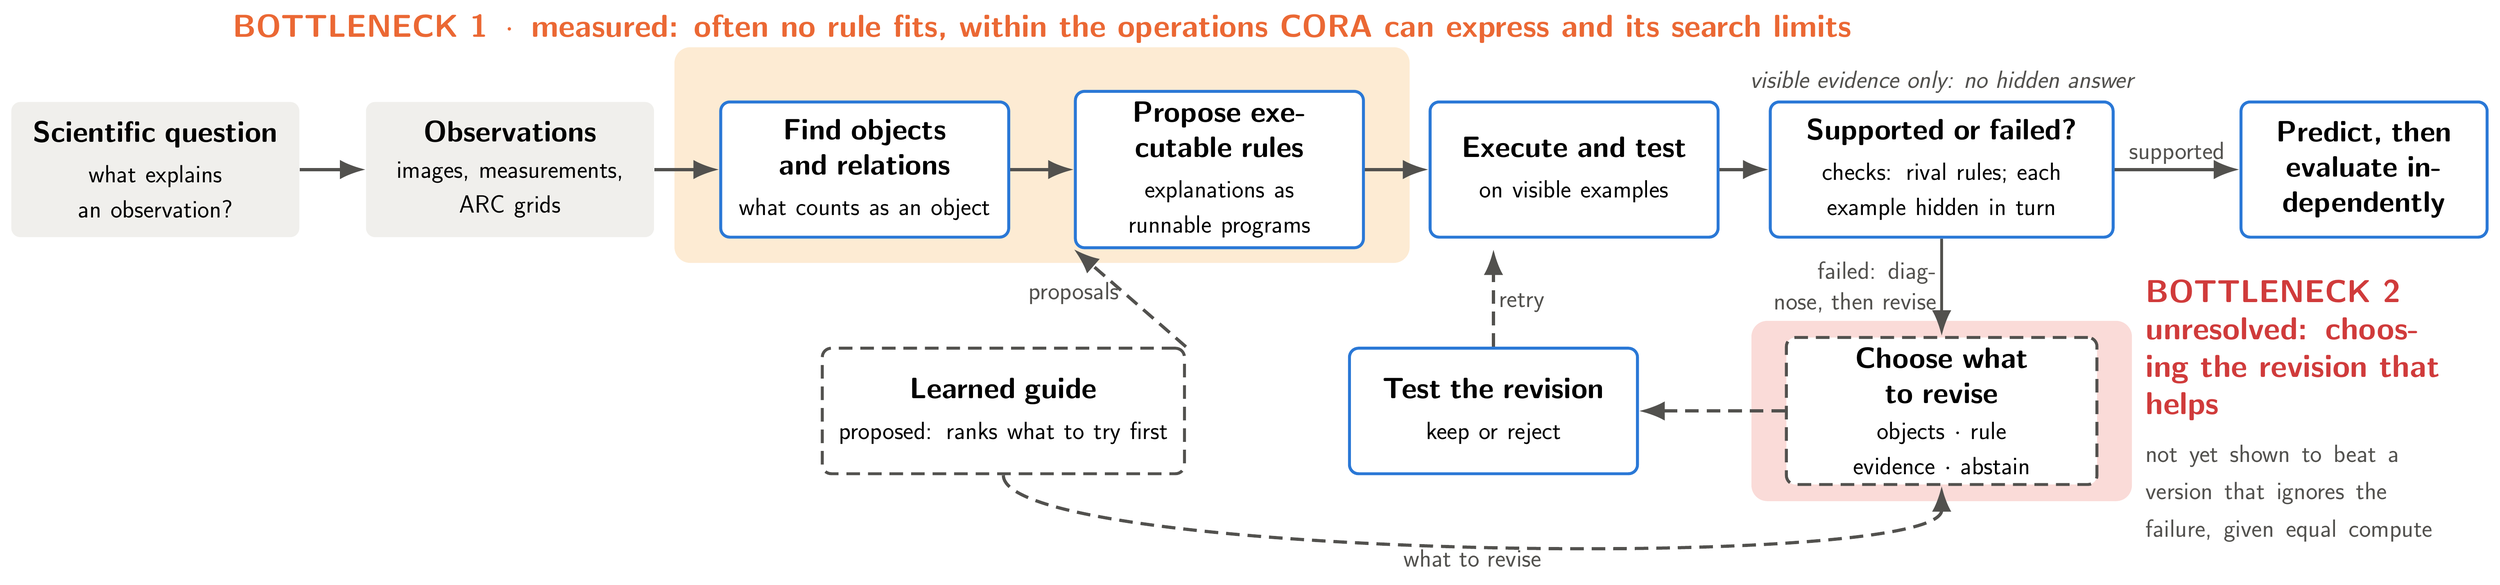
\begin{tikzpicture}[node distance=2.1cm]
  \tikzset{main/.style={text width=8.3cm, minimum height=4.2cm}}
  % bottleneck bands (drawn first, behind the nodes)
  \fill[band1, rounded corners=14pt] (-16.4,-2.9) rectangle (6.4,3.8);
  \node[font=\fontsize{28}{33}\selectfont\bfseries, text=warm, anchor=south] at (-5.0,3.8)
    {BOTTLENECK 1 \,$\cdot$\, measured: often no rule fits, within the operations CORA can express and its search limits};
  \fill[band2, rounded corners=14pt] (17.0,-10.3) rectangle (28.8,-4.7);
  \node[font=\fontsize{28}{33}\selectfont\bfseries, text=critical, anchor=west, text width=9.4cm, align=left]
    at (29.1,-7.5) {BOTTLENECK 2\\ unresolved: choosing the revision that helps\\[0.3em]{\fontsize{22}{27}\selectfont\mdseries\color{ink2} not yet shown to beat a version that ignores the failure, given equal compute}};
  % the main path
  \node[ctx, main] (q) at (-32.5,0) {\textbf{Scientific question}\\[0.2em]{\diagsub what explains an observation?}};
  \node[ctx, main] (o) at (-21.5,0) {\textbf{Observations}\\[0.2em]{\diagsub images, measurements,\\ ARC grids}};
  \node[stage, main] (f) at (-10.5,0) {\textbf{Find objects and relations}\\[0.2em]{\diagsub what counts as an object}};
  \node[stage, main] (p) at (0.5,0) {\textbf{Propose executable rules}\\[0.2em]{\diagsub explanations as runnable programs}};
  \node[stage, main] (e) at (11.5,0) {\textbf{Execute and test}\\[0.2em]{\diagsub on visible examples}};
  \node[stage, main, text width=10.0cm] (s) at (22.9,0) {\textbf{Supported or failed?}\\[0.2em]{\diagsub checks: rival rules; each example hidden in turn}};
  \node[stage, main, text width=7.0cm] (v) at (36.0,0) {\textbf{Predict, then evaluate independently}};
  \foreach \a/\b in {q/o, o/f, f/p, p/e, e/s} \draw[flow] (\a) -- (\b);
  \draw[flow] (s) -- node[lab, above] {supported} (v);
  % the revision loop
  \node[pstage, text width=9.0cm, minimum height=3.9cm] (r) at (22.9,-7.5)
    {\textbf{Choose what to revise}\\[0.2em]{\diagsub objects $\cdot$ rule\\ evidence $\cdot$ abstain}};
  \node[stage, text width=8.3cm, minimum height=3.9cm] (t) at (9.0,-7.5)
    {\textbf{Test the revision}\\[0.2em]{\diagsub keep or reject}};
  \draw[flow] (s) -- node[lab, left, text width=7.0cm, align=right] {failed: diagnose, then revise} (r);
  \draw[dflow] (r) -- (t);
  \draw[dflow] (t.north) -- node[lab, right, pos=0.45] {retry} (t.north |- p.south);
  % the proposed learned component, inside the loop
  \node[pstage, text width=10.6cm, minimum height=3.9cm] (l) at (-6.2,-7.5)
    {\textbf{Learned guide}\\[0.2em]{\diagsub proposed: ranks what to try first}};
  \draw[dflow] (l.north east) -- node[lab, left, pos=0.55] {proposals} (p.south west);
  \draw[dflow] (l.south) .. controls (-6.2,-12.1) and (22.9,-12.5) .. node[lab, below, pos=0.5] {what to revise} (r.south);
  \node[lab, font=\diagsub\itshape, anchor=south] at (22.9,2.25) {visible evidence only: no hidden answer};
\end{tikzpicture}
\par\vspace{0.4em}
{\secfont\color{ink2}
Solid: implemented and tested. Dashed: proposed. Grey: context. \textbf{Failed:} no rule fits, rivals disagree, or a hidden example
breaks the rule. \textbf{Exposed task:} one already studied during development. A tested revision is not
automatically a correct explanation.
\par}
\end{posterblock}

\begin{columns}

\column{0.333}
\begin{posterblock}{\bt{ARC is our controlled testbed}}
\bodyfont
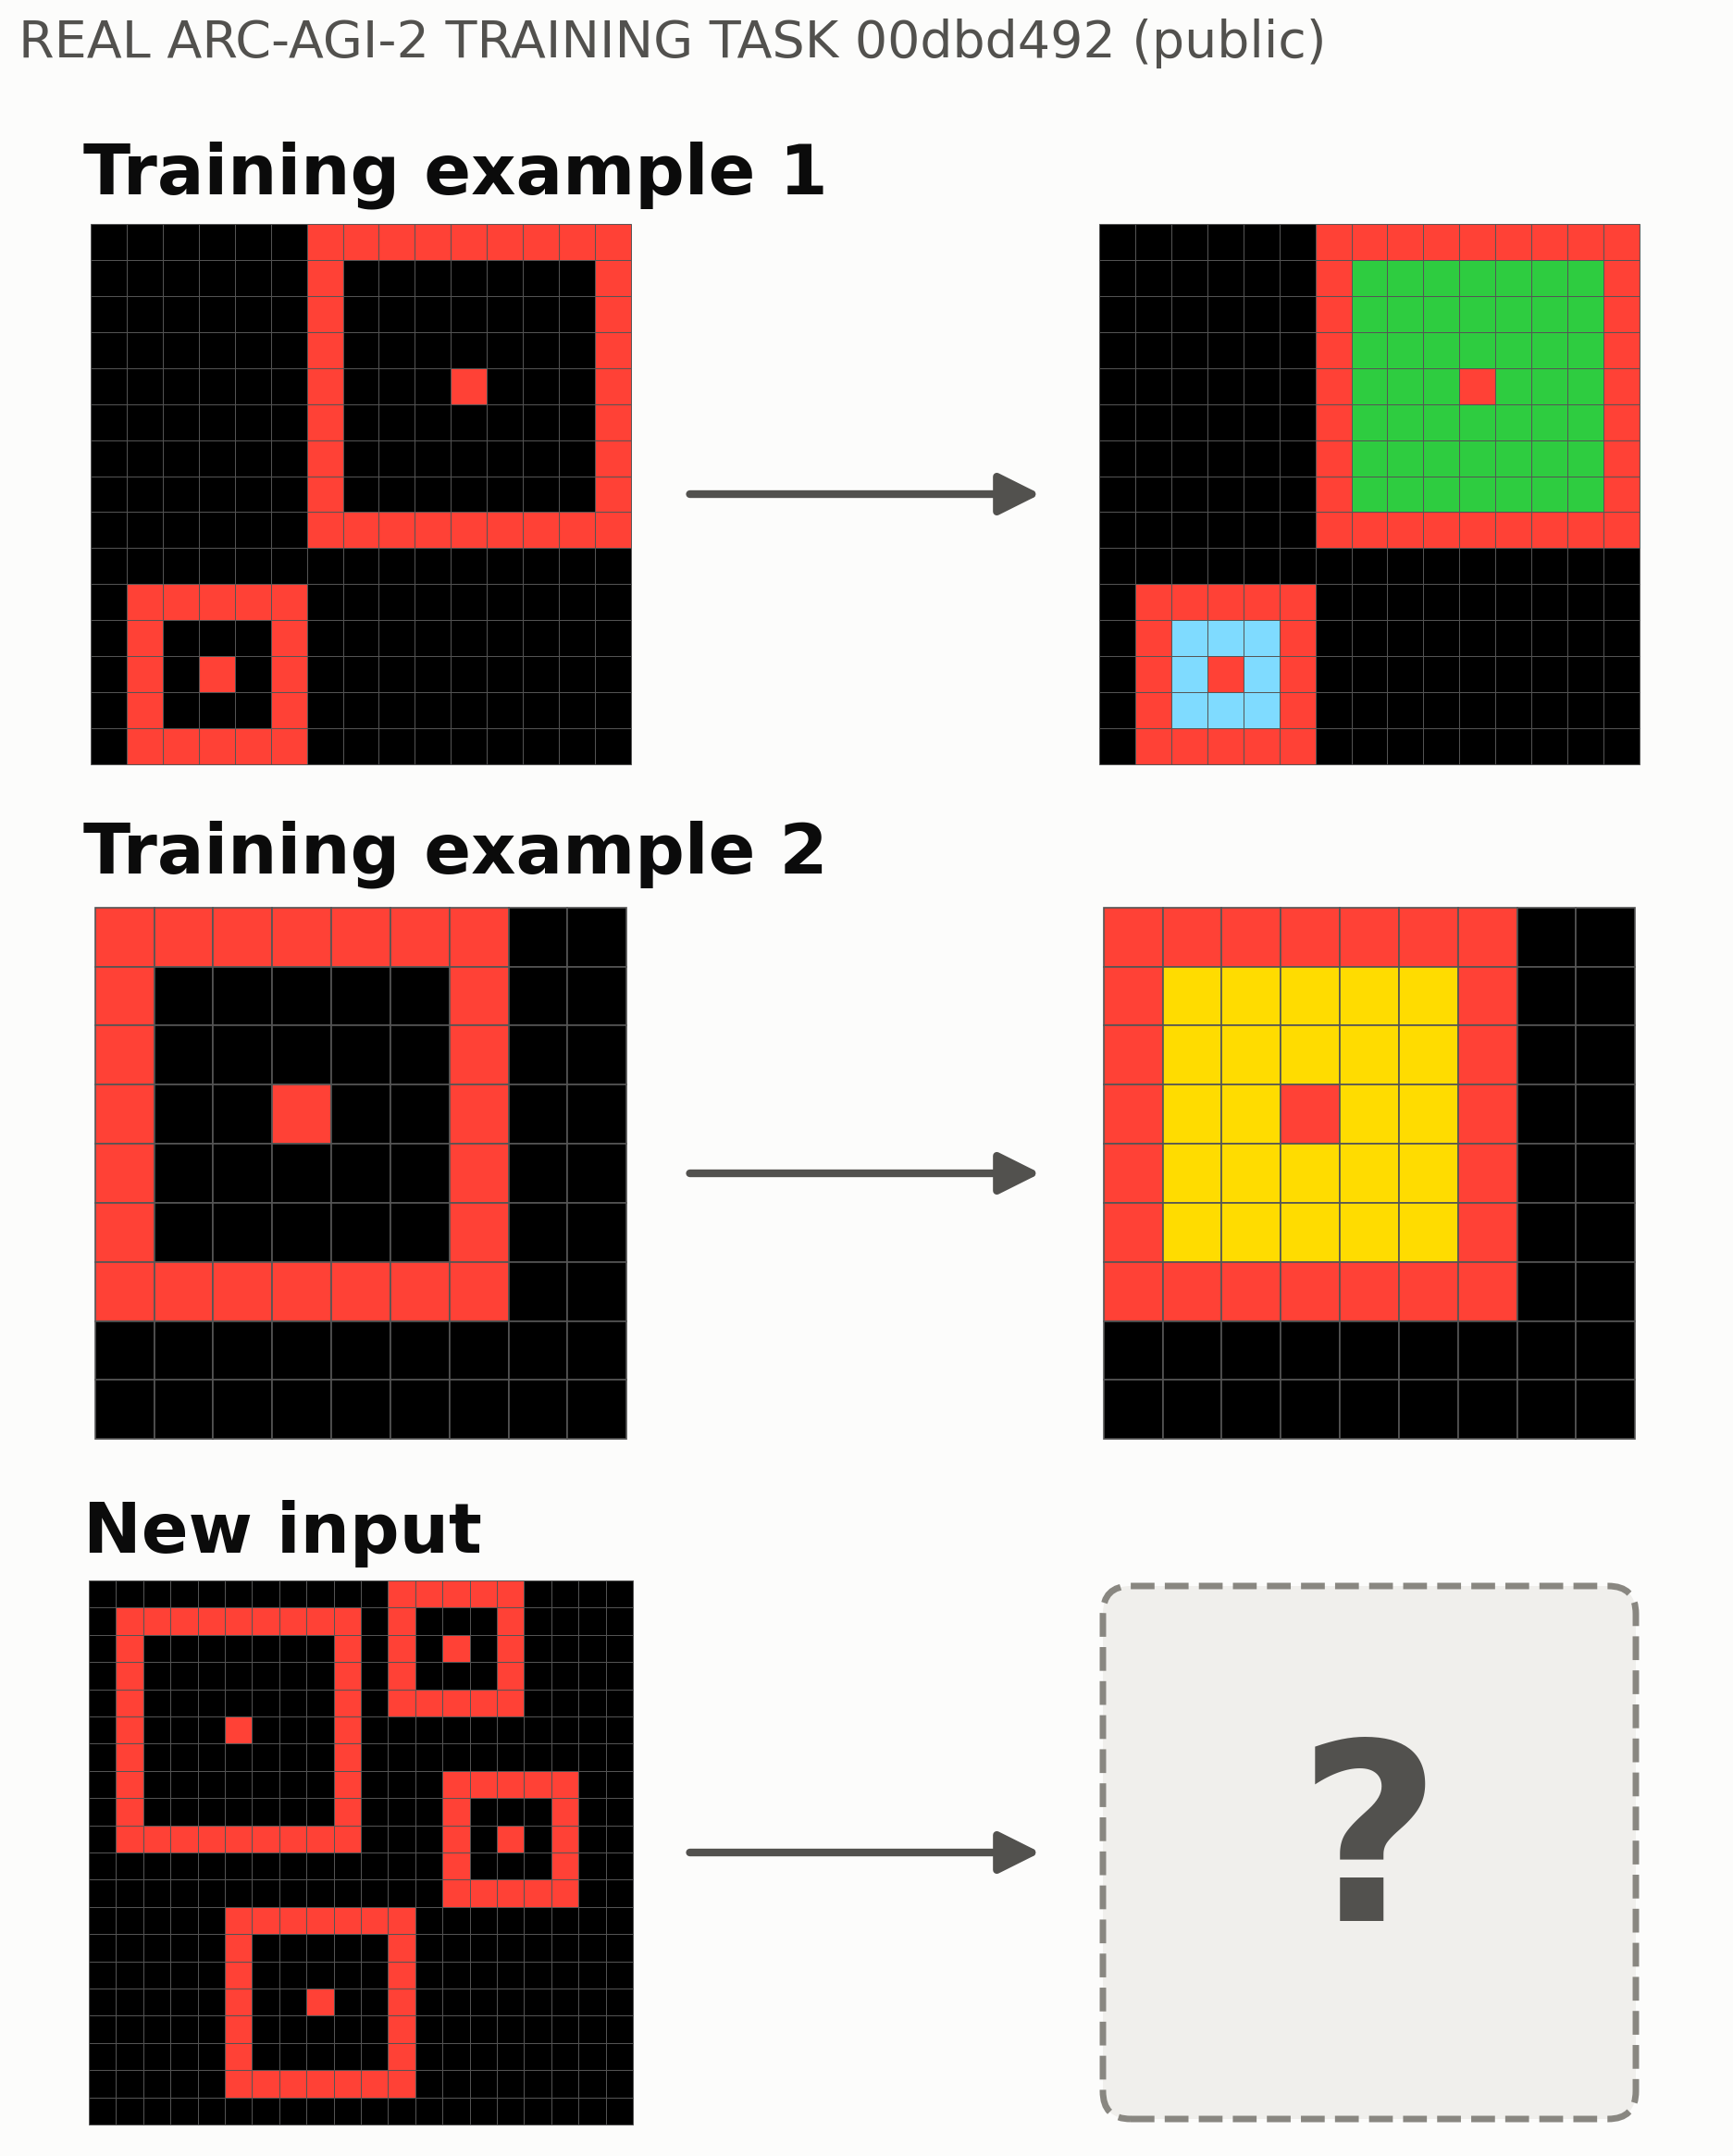
\includegraphics[width=\linewidth]{figures/fig_arc_intro_00dbd492_large.png}

{\secfont\color{ink2}
Rule: each frame's fill colour depends on its size.
\par}
\end{posterblock}

\begin{posterblock}{\bt{Why rules fail}}
\bodyfont
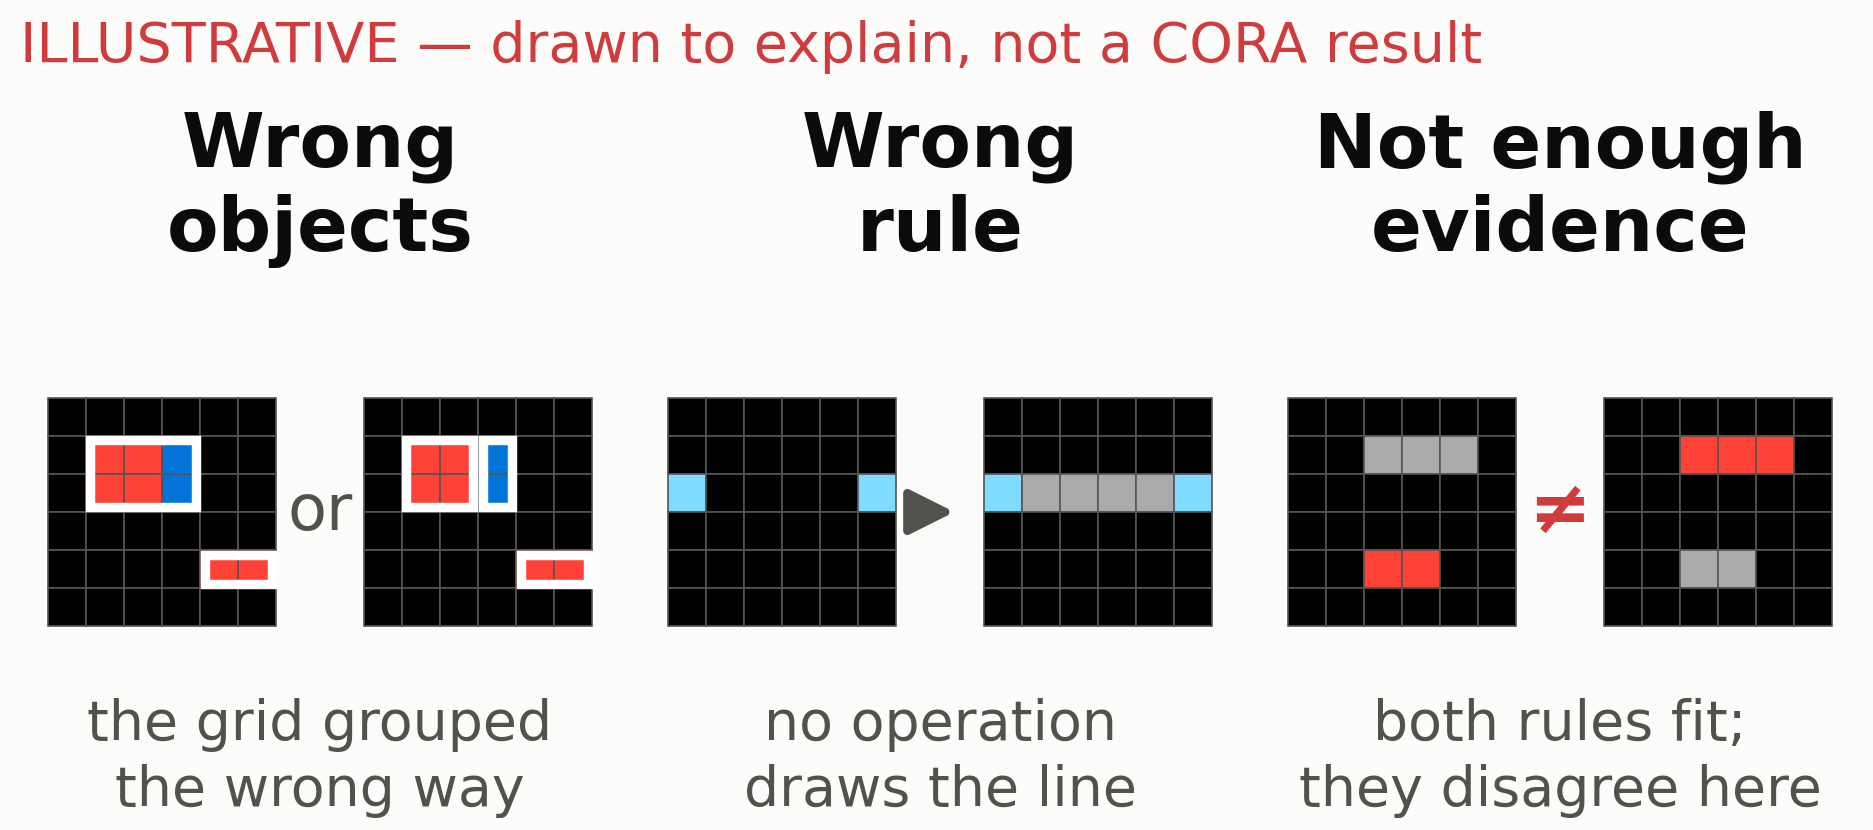
\includegraphics[width=\linewidth]{figures/fig_three_causes_row_ILLUSTRATIVE.png}

{\secfont\color{ink2}
Memorization: fits the examples, fails the new input.
\par}
\end{posterblock}

\column{0.333}
\begin{posterblock}{\bt{Done: a rule CORA built}\chip{good}{DONE, ONE TASK}}
\bodyfont
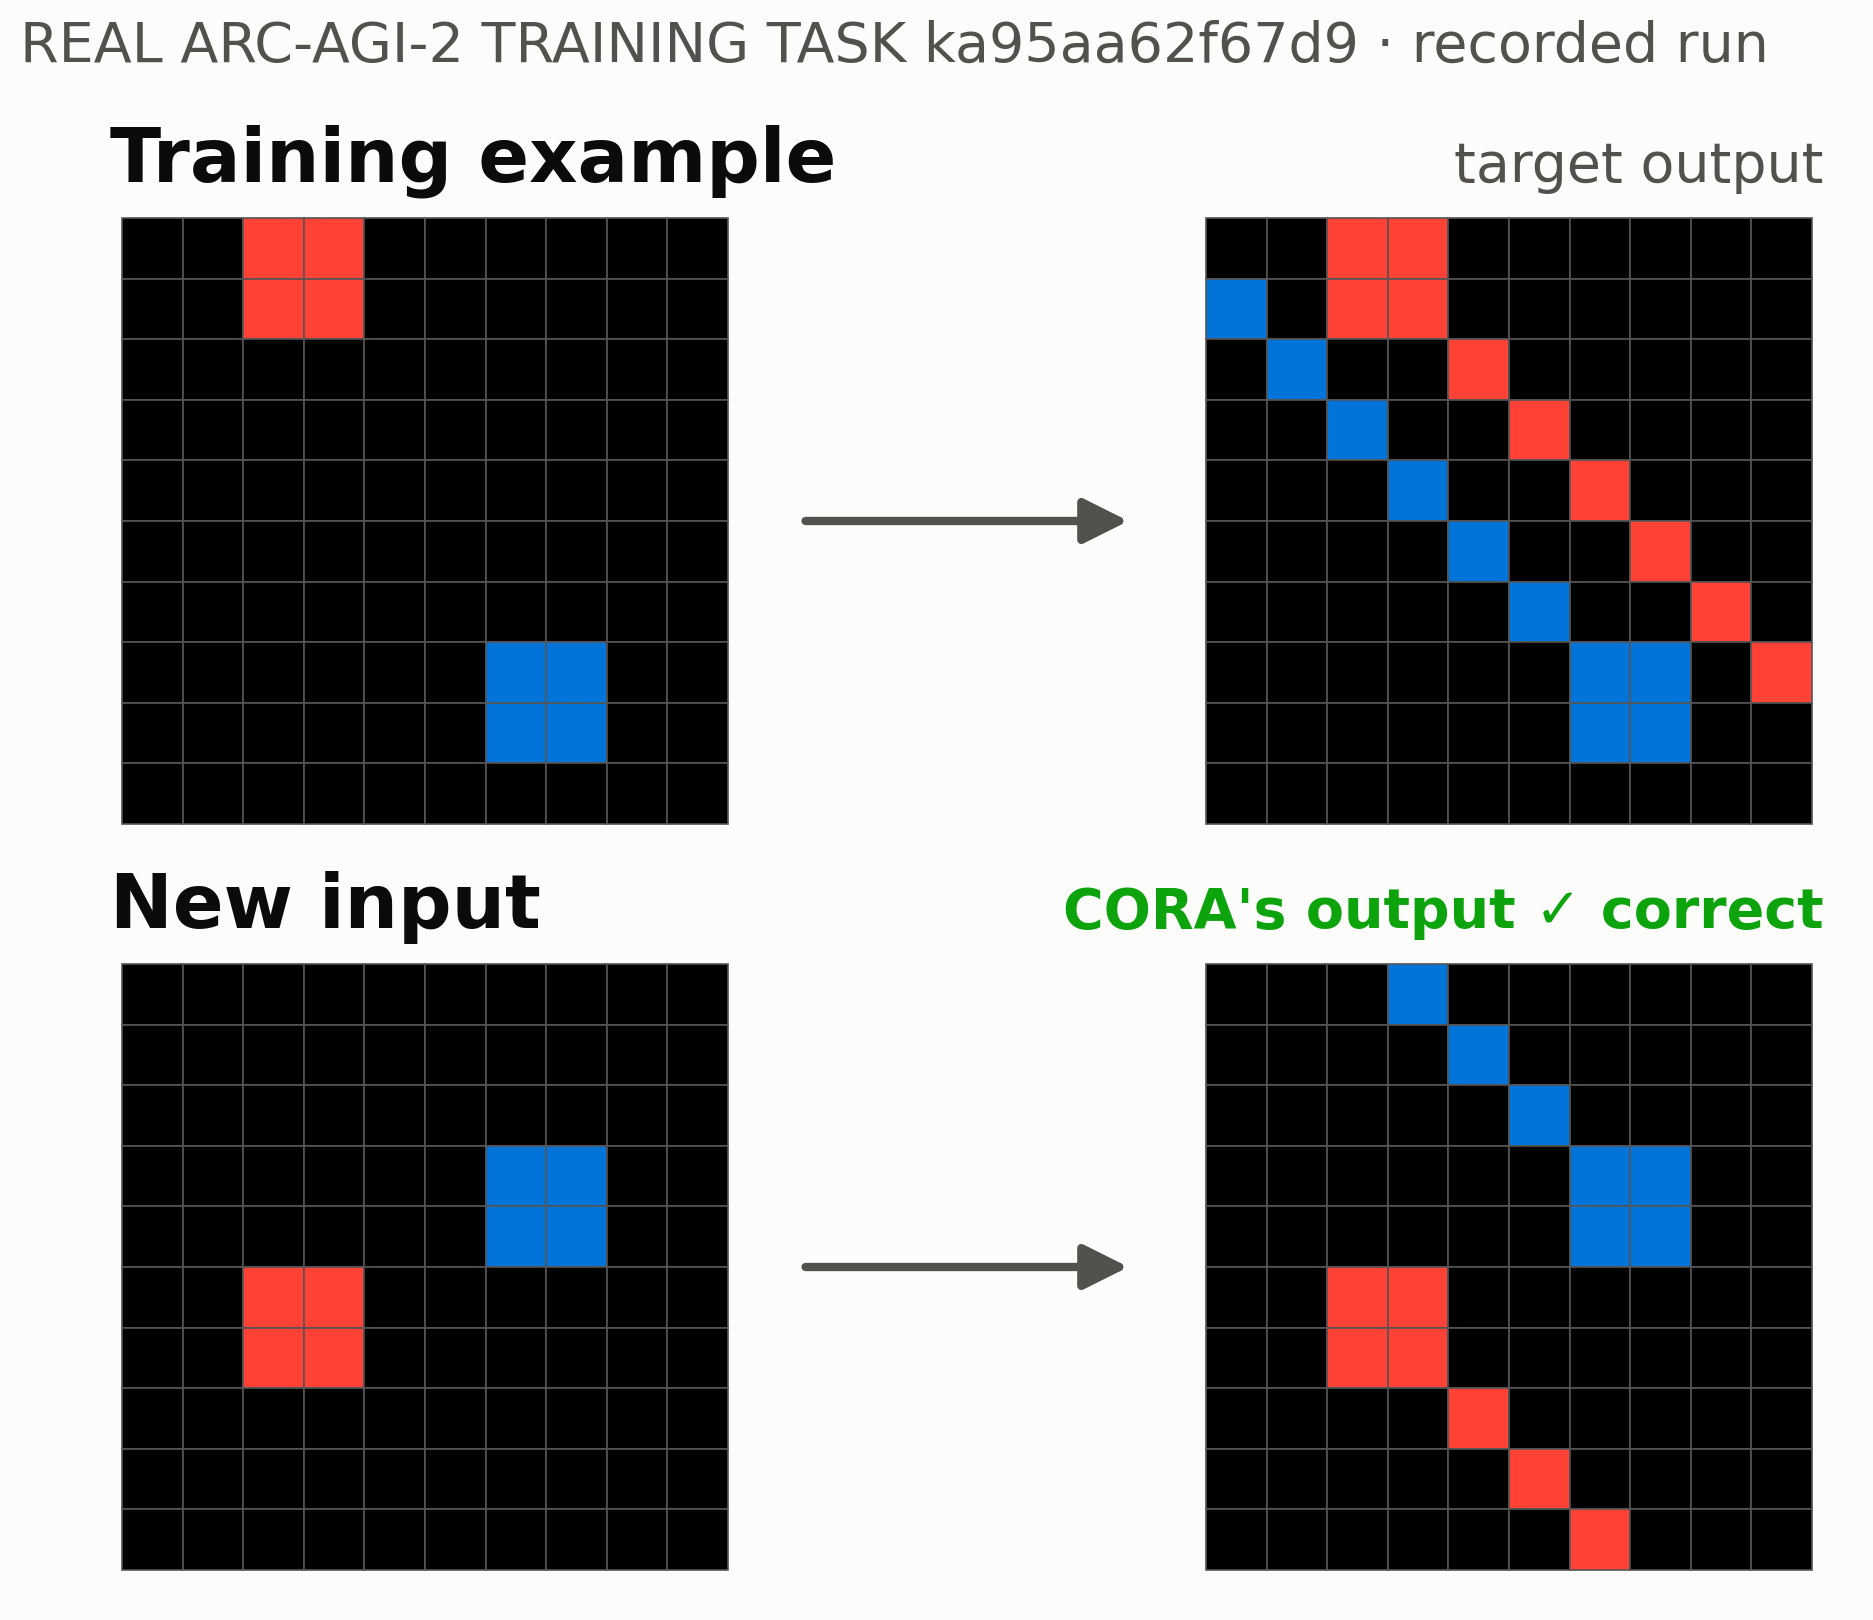
\includegraphics[width=\linewidth]{figures/fig_real_rule_ka95aa62f67d9_large.png}

\textbf{Rule:} {\color{arcblue}\textbf{blue}} objects send a line up-left; {\color{arcred}\textbf{red}} ones, down-right.\par\vspace{0.3em}{\secfont
Correct, and rebuilt 3 of 3 times with one example hidden, on an exposed task. A version that ignored the failure
record found it too.
\par}
\end{posterblock}

\begin{posterblock}{\bt{Where it fails}\chip{critical}{NEGATIVE}}
\bodyfont\centering{\color{critical}\bignum{0 / 58}}\par\vspace{0.1em}
new verified solutions from building rules
\par\vspace{0.2em}
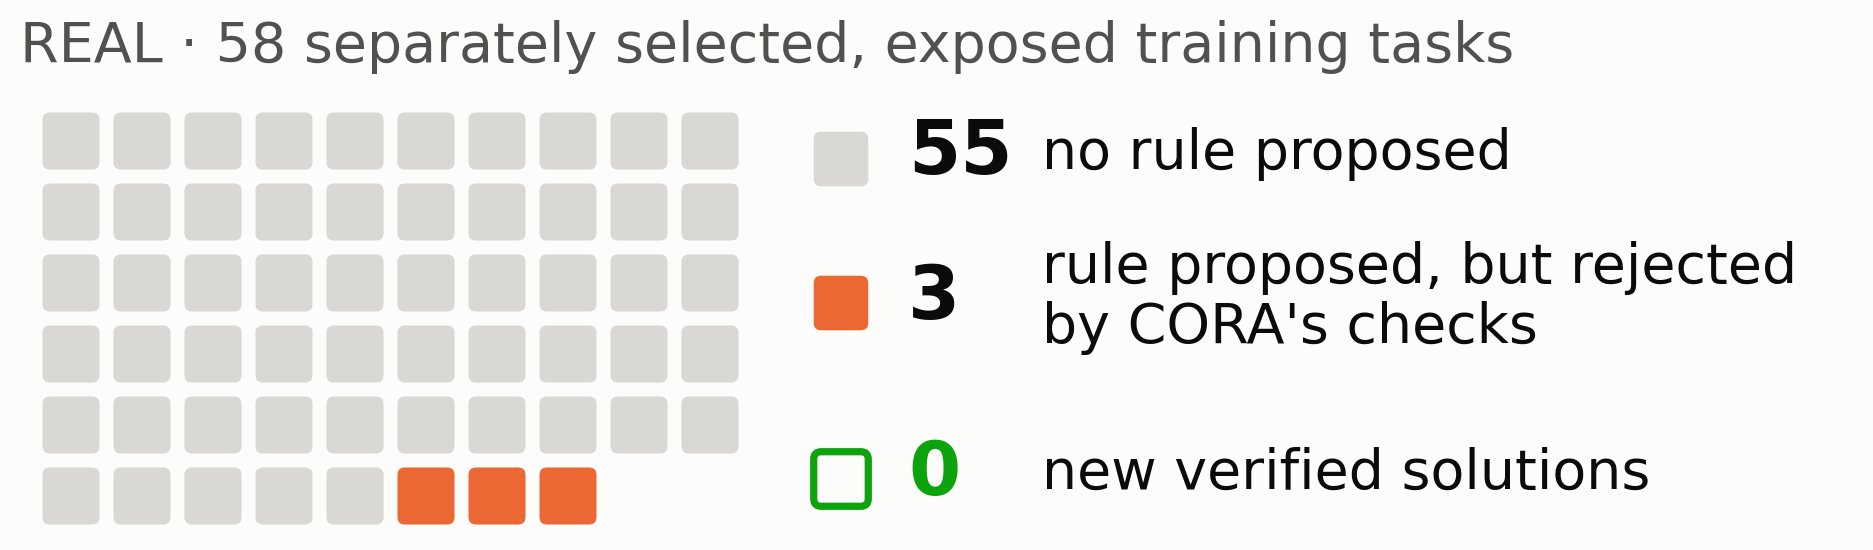
\includegraphics[width=\linewidth]{figures/fig_construction_58_outcomes.png}

\raggedright{\secfont\color{ink2}
With or without the failure record: 0; no wrong answers.
\par}
\end{posterblock}

\column{0.333}
\begin{posterblock}{\bt{Thin evidence, flagged}\chip{warm}{DEVELOPMENT}}
\bodyfont
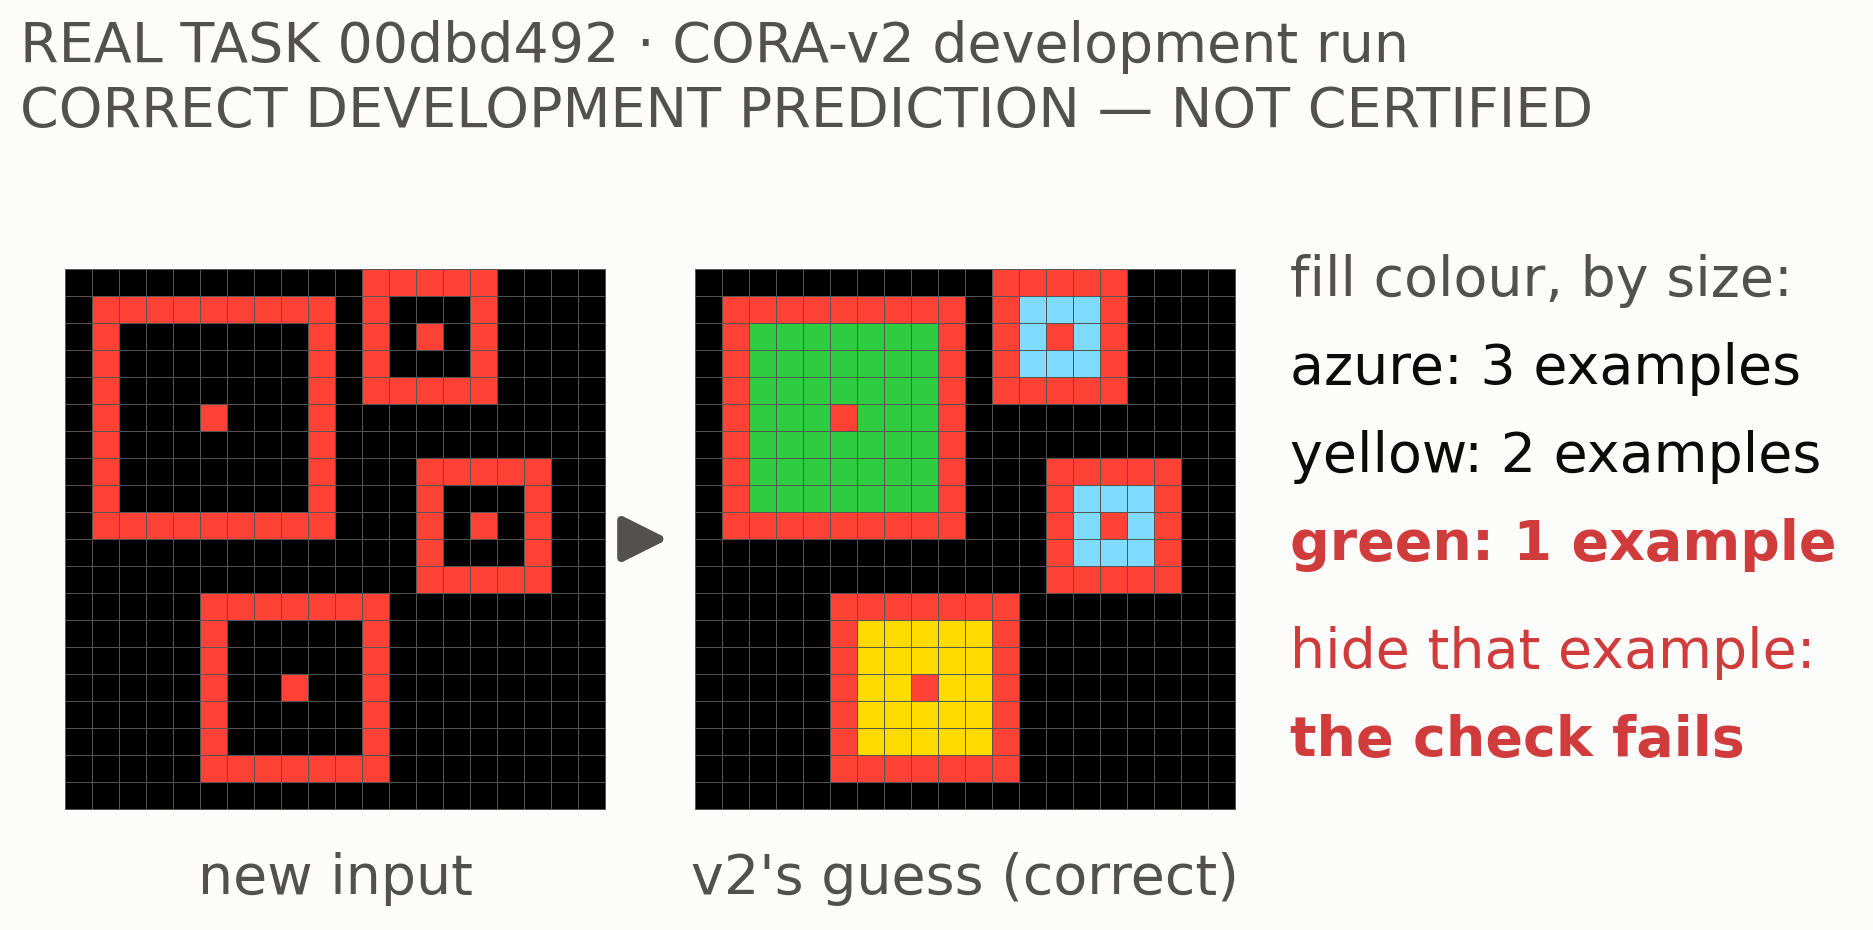
\includegraphics[width=\linewidth]{figures/fig_v2_uncertified_00dbd492_large.png}

{\secfont
Only one example shows the green fill, so CORA-v2, which keeps every fitting rule, does not certify its correct
guess. \textbf{Certified:} a unique rule that, rebuilt without any one example, still predicts it.
\par}
\end{posterblock}

\begin{posterblock}{\bt{Next: learning inside CORA}\chip{ink2}{PROPOSED}}
\centering
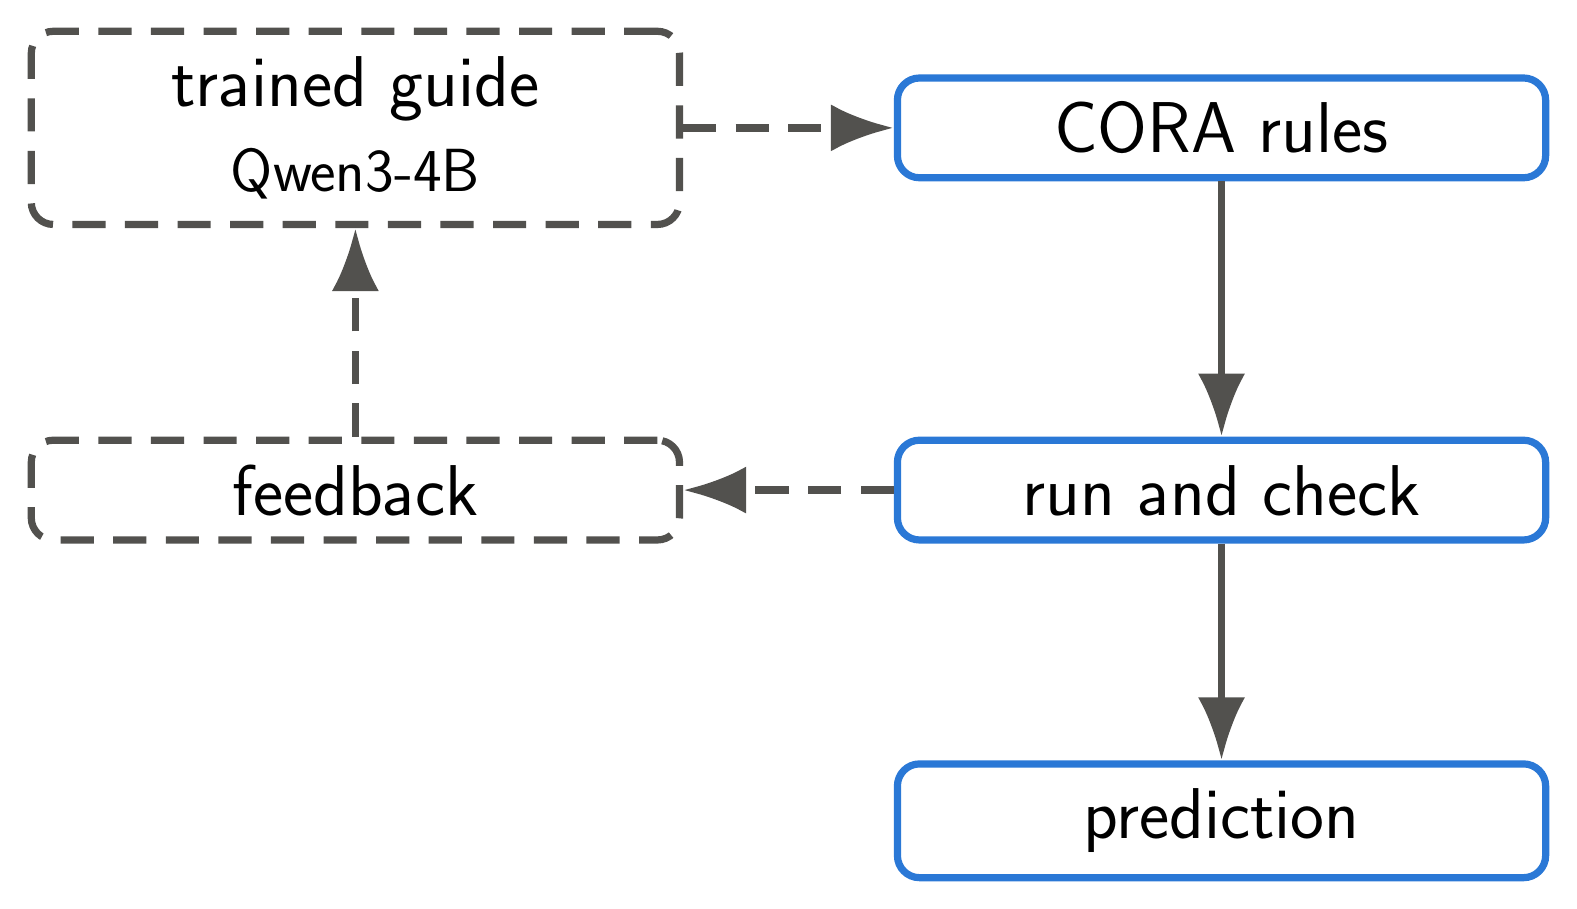
\begin{tikzpicture}
  \node[pstage, text width=7.6cm] (a) at (0,0) {trained guide\\{\diagsub Qwen3-4B}};
  \node[stage, text width=7.6cm] (b) at (11.0,0) {CORA rules};
  \node[stage, text width=7.6cm] (c) at (11.0,-4.6) {run and check};
  \node[pstage, text width=7.6cm] (d) at (0,-4.6) {feedback};
  \node[stage, text width=7.6cm] (e) at (11.0,-8.8) {prediction};
  \draw[dflow] (a) -- (b); \draw[flow] (b) -- (c); \draw[dflow] (c) -- (d); \draw[dflow] (d) -- (a); \draw[flow] (c) -- (e);
\end{tikzpicture}
\par\vspace{0.3em}
\bodyfont
A trained model would only rank what CORA tries first; CORA still checks every answer. No result yet.

\vspace{0.6em}{\secfont\color{ink2}
For scale: my reproduction of NVARC, a published Qwen3-4B method (not mine), scores 27.64\% on Kaggle's public
leaderboard; CORA scores 0.00\%.
\par}
\end{posterblock}

\end{columns}

\begin{posterblock}{}
{\fontsize{36}{44}\selectfont\bfseries\raggedright
If learning from failure works on ARC, test the same revision procedure---not ARC's grid operations---on biological
questions with independent validation. {\color{critical}[UNTESTED]}
\par}\vspace{0.4em}{\fontsize{22}{27}\selectfont\color{ink2}\raggedright
Prior work: Popper, DreamCoder, LILO, Model Discovery Agent (explainer). Numbers:
\texttt{records/CORA\_SUMMIT\_CLAIM\_LEDGER\_20261017.md}. Images: ISIC\_0000013, CC-0; maize leaf DSC\_0042, author's study, unpublished.
\par}
\end{posterblock}
\end{document}
